
%% bare_conf.tex
%% V1.4b
%% 2015/08/26
%% by Michael Shell
%% See:
%% http://www.michaelshell.org/
%% for current contact information.
%%
%% This is a skeleton file demonstrating the use of IEEEtran.cls
%% (requires IEEEtran.cls version 1.8b or later) with an IEEE
%% conference paper.
%%
%% Support sites:
%% http://www.michaelshell.org/tex/ieeetran/
%% http://www.ctan.org/pkg/ieeetran
%% and
%% http://www.ieee.org/

%%*************************************************************************
%% Legal Notice:
%% This code is offered as-is without any warranty either expressed or
%% implied; without even the implied warranty of MERCHANTABILITY or
%% FITNESS FOR A PARTICULAR PURPOSE! 
%% User assumes all risk.
%% In no event shall the IEEE or any contributor to this code be liable for
%% any damages or losses, including, but not limited to, incidental,
%% consequential, or any other damages, resulting from the use or misuse
%% of any information contained here.
%%
%% All comments are the opinions of their respective authors and are not
%% necessarily endorsed by the IEEE.
%%
%% This work is distributed under the LaTeX Project Public License (LPPL)
%% ( http://www.latex-project.org/ ) version 1.3, and may be freely used,
%% distributed and modified. A copy of the LPPL, version 1.3, is included
%% in the base LaTeX documentation of all distributions of LaTeX released
%% 2003/12/01 or later.
%% Retain all contribution notices and credits.
%% ** Modified files should be clearly indicated as such, including  **
%% ** renaming them and changing author support contact information. **
%%*************************************************************************


% *** Authors should verify (and, if needed, correct) their LaTeX system  ***
% *** with the testflow diagnostic prior to trusting their LaTeX platform ***
% *** with production work. The IEEE's font choices and paper sizes can   ***
% *** trigger bugs that do not appear when using other class files.       ***                          ***
% The testflow support page is at:
% http://www.michaelshell.org/tex/testflow/



\documentclass[conference]{IEEEtran}
% Some Computer Society conferences also require the compsoc mode option,
% but others use the standard conference format.
%
% If IEEEtran.cls has not been installed into the LaTeX system files,
% manually specify the path to it like:
% \documentclass[conference]{../sty/IEEEtran}





% Some very useful LaTeX packages include:
% (uncomment the ones you want to load)


% *** MISC UTILITY PACKAGES ***
%
%\usepackage{ifpdf}
% Heiko Oberdiek's ifpdf.sty is very useful if you need conditional
% compilation based on whether the output is pdf or dvi.
% usage:
% \ifpdf
%   % pdf code
% \else
%   % dvi code
% \fi
% The latest version of ifpdf.sty can be obtained from:
% http://www.ctan.org/pkg/ifpdf
% Also, note that IEEEtran.cls V1.7 and later provides a builtin
% \ifCLASSINFOpdf conditional that works the same way.
% When switching from latex to pdflatex and vice-versa, the compiler may
% have to be run twice to clear warning/error messages.






% *** CITATION PACKAGES ***
%
%\usepackage{cite}
% cite.sty was written by Donald Arseneau
% V1.6 and later of IEEEtran pre-defines the format of the cite.sty package
% \cite{} output to follow that of the IEEE. Loading the cite package will
% result in citation numbers being automatically sorted and properly
% "compressed/ranged". e.g., [1], \cite{seznec2007tage}, \cite{calder1997evidence}, \cite{lee1995branch}, \cite{jimenez2001dynamic}, \cite{jimenez2003fast} without using
% cite.sty will become [1], \cite{calder1997evidence}, \cite{jimenez2001dynamic}--\cite{lee1995branch}, \cite{seznec2007tage} using cite.sty. cite.sty's
% \cite will automatically add leading space, if needed. Use cite.sty's
% noadjust option (cite.sty V3.8 and later) if you want to turn this off
% such as if a citation ever needs to be enclosed in parenthesis.
% cite.sty is already installed on most LaTeX systems. Be sure and use
% version 5.0 (2009-03-20) and later if using hyperref.sty.
% The latest version can be obtained at:
% http://www.ctan.org/pkg/cite
% The documentation is contained in the cite.sty file itself.






% *** GRAPHICS RELATED PACKAGES ***
%
\ifCLASSINFOpdf
  % \usepackage[pdftex]{graphicx}
  % declare the path(s) where your graphic files are
  % \graphicspath{{../pdf/}{../jpeg/}}
  % and their extensions so you won't have to specify these with
  % every instance of \includegraphics
  % \DeclareGraphicsExtensions{.pdf,.jpeg,.png}
\else
  % or other class option (dvipsone, dvipdf, if not using dvips). graphicx
  % will default to the driver specified in the system graphics.cfg if no
  % driver is specified.
  % \usepackage[dvips]{graphicx}
  % declare the path(s) where your graphic files are
  % \graphicspath{{../eps/}}
  % and their extensions so you won't have to specify these with
  % every instance of \includegraphics
  % \DeclareGraphicsExtensions{.eps}
\fi
% graphicx was written by David Carlisle and Sebastian Rahtz. It is
% required if you want graphics, photos, etc. graphicx.sty is already
% installed on most LaTeX systems. The latest version and documentation
% can be obtained at: 
% http://www.ctan.org/pkg/graphicx
% Another good source of documentation is "Using Imported Graphics in
% LaTeX2e" by Keith Reckdahl which can be found at:
% http://www.ctan.org/pkg/epslatex
%
% latex, and pdflatex in dvi mode, support graphics in encapsulated
% postscript (.eps) format. pdflatex in pdf mode supports graphics
% in .pdf, .jpeg, .png and .mps (metapost) formats. Users should ensure
% that all non-photo figures use a vector format (.eps, .pdf, .mps) and
% not a bitmapped formats (.jpeg, .png). The IEEE frowns on bitmapped formats
% which can result in "jaggedy"/blurry rendering of lines and letters as
% well as large increases in file sizes.
%
% You can find documentation about the pdfTeX application at:
% http://www.tug.org/applications/pdftex





% *** MATH PACKAGES ***
%
%\usepackage{amsmath}
% A popular package from the American Mathematical Society that provides
% many useful and powerful commands for dealing with mathematics.
%
% Note that the amsmath package sets \interdisplaylinepenalty to 10000
% thus preventing page breaks from occurring within multiline equations. Use:
%\interdisplaylinepenalty=2500
% after loading amsmath to restore such page breaks as IEEEtran.cls normally
% does. amsmath.sty is already installed on most LaTeX systems. The latest
% version and documentation can be obtained at:
% http://www.ctan.org/pkg/amsmath





% *** SPECIALIZED LIST PACKAGES ***
%
%\usepackage{algorithmic}
% algorithmic.sty was written by Peter Williams and Rogerio Brito.
% This package provides an algorithmic environment fo describing algorithms.
% You can use the algorithmic environment in-text or within a figure
% environment to provide for a floating algorithm. Do NOT use the algorithm
% floating environment provided by algorithm.sty (by the same authors) or
% algorithm2e.sty (by Christophe Fiorio) as the IEEE does not use dedicated
% algorithm float types and packages that provide these will not provide
% correct IEEE style captions. The latest version and documentation of
% algorithmic.sty can be obtained at:
% http://www.ctan.org/pkg/algorithms
% Also of interest may be the (relatively newer and more customizable)
% algorithmicx.sty package by Szasz Janos:
% http://www.ctan.org/pkg/algorithmicx




% *** ALIGNMENT PACKAGES ***
%
%\usepackage{array}
% Frank Mittelbach's and David Carlisle's array.sty patches and improves
% the standard LaTeX2e array and tabular environments to provide better
% appearance and additional user controls. As the default LaTeX2e table
% generation code is lacking to the point of almost being broken with
% respect to the quality of the end results, all users are strongly
% advised to use an enhanced (at the very least that provided by array.sty)
% set of table tools. array.sty is already installed on most systems. The
% latest version and documentation can be obtained at:
% http://www.ctan.org/pkg/array


% IEEEtran contains the IEEEeqnarray family of commands that can be used to
% generate multiline equations as well as matrices, tables, etc., of high
% quality.




% *** SUBFIGURE PACKAGES ***
%\ifCLASSOPTIONcompsoc
%  \usepackage[caption=false,font=normalsize,labelfont=sf,textfont=sf]{subfig}
%\else
%  \usepackage[caption=false,font=footnotesize]{subfig}
%\fi
% subfig.sty, written by Steven Douglas Cochran, is the modern replacement
% for subfigure.sty, the latter of which is no longer maintained and is
% incompatible with some LaTeX packages including fixltx2e. However,
% subfig.sty requires and automatically loads Axel Sommerfeldt's caption.sty
% which will override IEEEtran.cls' handling of captions and this will result
% in non-IEEE style figure/table captions. To prevent this problem, be sure
% and invoke subfig.sty's "caption=false" package option (available since
% subfig.sty version 1.3, 2005/06/28) as this is will preserve IEEEtran.cls
% handling of captions.
% Note that the Computer Society format requires a larger sans serif font
% than the serif footnote size font used in traditional IEEE formatting
% and thus the need to invoke different subfig.sty package options depending
% on whether compsoc mode has been enabled.
%
% The latest version and documentation of subfig.sty can be obtained at:
% http://www.ctan.org/pkg/subfig




% *** FLOAT PACKAGES ***
%
%\usepackage{fixltx2e}
% fixltx2e, the successor to the earlier fix2col.sty, was written by
% Frank Mittelbach and David Carlisle. This package corrects a few problems
% in the LaTeX2e kernel, the most notable of which is that in current
% LaTeX2e releases, the ordering of single and double column floats is not
% guaranteed to be preserved. Thus, an unpatched LaTeX2e can allow a
% single column figure to be placed prior to an earlier double column
% figure.
% Be aware that LaTeX2e kernels dated 2015 and later have fixltx2e.sty's
% corrections already built into the system in which case a warning will
% be issued if an attempt is made to load fixltx2e.sty as it is no longer
% needed.
% The latest version and documentation can be found at:
% http://www.ctan.org/pkg/fixltx2e


%\usepackage{stfloats}
% stfloats.sty was written by Sigitas Tolusis. This package gives LaTeX2e
% the ability to do double column floats at the bottom of the page as well
% as the top. (e.g., "\begin{figure*}[!b]" is not normally possible in
% LaTeX2e). It also provides a command:
%\fnbelowfloat
% to enable the placement of footnotes below bottom floats (the standard
% LaTeX2e kernel puts them above bottom floats). This is an invasive package
% which rewrites many portions of the LaTeX2e float routines. It may not work
% with other packages that modify the LaTeX2e float routines. The latest
% version and documentation can be obtained at:
% http://www.ctan.org/pkg/stfloats
% Do not use the stfloats baselinefloat ability as the IEEE does not allow
% \baselineskip to stretch. Authors submitting work to the IEEE should note
% that the IEEE rarely uses double column equations and that authors should try
% to avoid such use. Do not be tempted to use the cuted.sty or midfloat.sty
% packages (also by Sigitas Tolusis) as the IEEE does not format its papers in
% such ways.
% Do not attempt to use stfloats with fixltx2e as they are incompatible.
% Instead, use Morten Hogholm'a dblfloatfix which combines the features
% of both fixltx2e and stfloats:
%
% \usepackage{dblfloatfix}
% The latest version can be found at:
% http://www.ctan.org/pkg/dblfloatfix




% *** PDF, URL AND HYPERLINK PACKAGES ***
%
%\usepackage{url}
% url.sty was written by Donald Arseneau. It provides better support for
% handling and breaking URLs. url.sty is already installed on most LaTeX
% systems. The latest version and documentation can be obtained at:
% http://www.ctan.org/pkg/url
% Basically, \url{my_url_here}.
\usepackage{algorithm}
\usepackage{algpseudocode}
\usepackage{amsmath}
\usepackage{amsmath,amssymb,amsthm,latexsym,paralist, booktabs}
\usepackage{url}
\usepackage[pdftex]{graphicx}
% default pic path
\graphicspath{{pics/}}




% *** Do not adjust lengths that control margins, column widths, etc. ***
% *** Do not use packages that alter fonts (such as pslatex).         ***
% There should be no need to do such things with IEEEtran.cls V1.6 and later.
% (Unless specifically asked to do so by the journal or conference you plan
% to submit to, of course. )


% correct bad hyphenation here
\hyphenation{op-tical net-works semi-conduc-tor}


\begin{document}
%
% paper title
% Titles are generally capitalized except for words such as a, an, and, as,
% at, but, by, for, in, nor, of, on, or, the, to and up, which are usually
% not capitalized unless they are the first or last word of the title.
% Linebreaks \\ can be used within to get better formatting as desired.
% Do not put math or special symbols in the title.
\title{Yet Another Implementation of Fast Path-Based Neural Branch Predictor}


% author names and affiliations
% use a multiple column layout for up to three different
% affiliations
\author{\IEEEauthorblockN{Yukun Zeng}
\IEEEauthorblockA{Department of Computer Science and Engineering\\
Texas A\&M University\\
College Station, TX 77840\\
Email: yzeng@tamu.edu}}

% conference papers do not typically use \thanks and this command
% is locked out in conference mode. If really needed, such as for
% the acknowledgment of grants, issue a \IEEEoverridecommandlockouts
% after \documentclass

% for over three affiliations, or if they all won't fit within the width
% of the page, use this alternative format:
% 
%\author{\IEEEauthorblockN{Michael Shell\IEEEauthorrefmark{1},
%Homer Simpson\IEEEauthorrefmark{2},
%James Kirk\IEEEauthorrefmark{3}, 
%Montgomery Scott\IEEEauthorrefmark{3} and
%Eldon Tyrell\IEEEauthorrefmark{4}}
%\IEEEauthorblockA{\IEEEauthorrefmark{1}School of Electrical and Computer Engineering\\
%Georgia Institute of Technology,
%Atlanta, Georgia 30332--0250\\ Email: see http://www.michaelshell.org/contact.html}
%\IEEEauthorblockA{\IEEEauthorrefmark{2}Twentieth Century Fox, Springfield, USA\\
%Email: homer@thesimpsons.com}
%\IEEEauthorblockA{\IEEEauthorrefmark{3}Starfleet Academy, San Francisco, California 96678-2391\\
%Telephone: (800) 555--1212, Fax: (888) 555--1212}
%\IEEEauthorblockA{\IEEEauthorrefmark{4}Tyrell Inc., 123 Replicant Street, Los Angeles, California 90210--4321}}




% use for special paper notices
%\IEEEspecialpapernotice{(Invited Paper)}




% make the title area
\maketitle

% As a general rule, do not put math, special symbols or citations
% in the abstract
\begin{abstract}
Branch prediction is an important technique used to improve instruction-level parallelism in deeply pipelined processors of modern parallel computer systems. In the last decade, a new approach of neural branch prediction was introduced and received increasing attention. Comparing to static branch prediction and some popular dynamic prediction strategies like two-level branch prediction and gshare, neural predictors generally achieve higher average performance in terms of hit rate but are also more complex in hardware implementation. In this paper, we review the branch prediction literature and present an implementation of Fast Path-Based Neural Branch Prediction, which is the simpliest neural approach that can also achieve considerable performance. The final benchmark show that our predictor outperforms gshare by 22.4\% under a 8KB hardware budget.
\end{abstract}

% no keywords




% For peer review papers, you can put extra information on the cover
% page as needed:
% \ifCLASSOPTIONpeerreview
% \begin{center} \bfseries EDICS Category: 3-BBND \end{center}
% \fi
%
% For peerreview papers, this IEEEtran command inserts a page break and
% creates the second title. It will be ignored for other modes.
\IEEEpeerreviewmaketitle



\section{Introduction}
% no \IEEEPARstart
In the instruction set of modern CPU, there are lots of basic instructions that functions differently. Through combining these basic instructions together in certain sequences, we can program the CPU to do complex computations and solve real-life problems. However, for complex applications, it's impossible that they can be solved by computing all the way to end, those applications are always involved with some if/loop logics. Thus, except for computation instructions like ADD, MULTIPLY, etc, there are also certain kinds of instructions exist to control the instruction flow and select next instruction to execute on-the-fly. Though branch instructions enable us to integrate more daily logics into computer programs, it might at the meantime break the smooth flow of instruction fetching and execution in highly parallel computer systems \cite{smith1981study}. Such problems result in delay since the result of a branch instruction changes the location of instruction fetches and the execution of next instruction must wait until the conditional branch decisions are made. To reduce such delays, branch predictors are introduced in \cite{smith1981study} to determine the next instruction that a branch instruction might lead to before it was executed. With branch prediction, we can start fetching, decoding and even executing the next instruction beforehand, which substantially improved the performance of modern pipelined microprocessors.
% You must have at least 2 lines in the paragraph with the drop letter
% (should never be an issue)

\section{Related Works}
Generally, the former researches conducted on Branch Prediction can be divided into two categories, static branch prediction and dynamic branch prediction. Here we present a brief review of predictors of those two types.

\subsection{Static Branch Prediction}
Static branch prediction is the earliest and simplest branch prediction strategy. As the name itself shows, such predictors produce static results, i.e., they made prediction decisions before program runtime. Classic static branch prediction strategies include but not limited to:
\begin{itemize}
	\item Predict all branches will be taken.
	\item Predict that all branches with certain operation code will be taken, others not taken.
	\item Predict all backward branches (toward lower addresses) will be taken, while all forward branches will not be taken.
\end{itemize}
Despite their simplicity, the actual performance of those strategies is considerably good, the result accuracy ranges from 60\% to more than 90\% depending on different benchmarks used \cite{smith1981study}. Afterwards, more static branch predictors are proposed, one typical example among them is static branch predictor with neural networks. Using this approach, the branch direction is predicted in compile-time by program features, its prediction results reached an 80\% correct prediction rate \cite{calder1997evidence}.

\subsection{Dynamic Branch Prediction}
Dynamic branch prediction makes prediction decisions based on history branch taken data. Since dynamic predictors can be self-tuning in the runtime, they can provide better performance most of the time. Typical dynamic predictors include:
\begin{itemize}
	\item Branch Target Buffer \cite{lee1995branch}: use 2-bit saturating up-down counters to collect history information for predictions.
	\item Two-level adaptive training branch prediction \cite{yeh1991two}: the most widely-used strategy that has been put in many real computer architecture.
	\item Dynamic Perceptron Branch Prediction(DPBP) \cite{jimenez2001dynamic}: first successful integration of neural networks into dynamic branch prediction.
	\item Path-Based Neural Branch Prediction(PBNBP) \cite{jimenez2003fast} and Piecewise Linear Branch Prediction(PLBP) \cite{jimenez2005idealized}: improved versions based on perceptron approach.
	\item L-TAGE \cite{seznec2007tage}: state-of-the-art branch prediction with high accuracy.
\end{itemize}

\section{The Path-Based Neural Predictor}
After careful evaluation of other branch prediction methods, I finally decided to choose PBNBP as my target. In the next two sections, I will state the reason of choosing this approach and present a review of its design.
\subsection{Reason}
Reviewed the evolution of branch predictors, I first decided to implement a dynamic predictor instead of static ones, the reasons shall be three fold:
\begin{itemize}
	\item Static prediction strategies in general perform worse than dynamic techniques.
	\item Static predictors are unable to tune themselves on the fly, while the prediction strategies always vary greatly between different programs.
	\item The program logic of static predictors is often simple and unchallenging.
\end{itemize}

When choosing dynamic branch predictors, I first narrowed down several high-quality research papers, which are perceptron, PBNBP, piecewise linear branch prediction and L-TAGE, among which perceptron is the earliest, L-TAGE performs the best and the other two is improved strategies based on or inspired by perceptron. After consulting Prof. Jiménez, I choose Path-Based Neural Branch Prediction approach for following reasons:
\begin{itemize}
	\item The paper of L-TAGE is too vague to understand, making it hard to implement in a short time.
	\item Perceptron as the precursor of dynamic neural network branch prediction is too simple and its performance might not help me win the prize.
	\item PLBP's requirements on memory space make it hard to satisfy the competition requirements. The size of a version of PLBP (which our professor used in a competition) is 65,789, which exceeds our project requirements \cite{jimenez2005idealized}. 
	\item PBNBP approach has a considerably good accuracy and enjoys a low latency, while occupying a reasonable space. PBNBP is easy to implement both in program and on hardware, which means it's highly applicable.
\end{itemize}

\begin{table}[!htp]
  \centering
  \caption{Algorithm Symbol Table}
  \label{symbol_tb}
  \begin{tabular}{cc}
    \toprule
    Symbol & Explanation\\
    \midrule
    $w$ & weight matrix for perceptron\\
    $i$ & index in rows of weight matrix $w$\\
    $n$ & design parameter\\
    $v$ & addresses of modulo n historical predicted branches\\
    $sv$ & speculative version of $v$\\
    $r$ & partial sum from last prediction\\
    $sr$ & speculative version of $r$\\
    $g$ & shift global history register\\
    $sg$ & speculative version of $g$\\
    $y$ & perceptron output\\
    $h$ & history length\\
    $outcome$ & the branch result of real execution\\
    $\theta$ & perceptron threshold\\
  	\bottomrule
  \end{tabular}
\end{table}

\begin{algorithm}[!htp]
  \caption{\textsc{Branch Predict}}
  \label{predict_algo}
  \begin{algorithmic}
  \Function{Predict}{address}
	\State $i=address \mod n$
	\State $shift(sv, i)$
	\State $update.v=sv$
	\State $update.g=sg$
	\State $y=w[i, 0]+sr[h]$
	\State $prediction=(y>=0)$
	\For{$j=1\rightarrow h$}
		\State $k=h-j$
		\If{$prediction=taken$}
			\State $sr[k+1]=sr[k]+w[i, j]$
		\Else
			\State $sr[k+1]=sr[k]-w[i, j]$
		\EndIf
	\EndFor
      \State $sr[0] = 0$
      \State $shift(sg, prediction)$

      \State $update.i = i$
      \State $update.y = y$
      \State $update.prediction=prediction$
      \State \Return $update$
  \EndFunction
  \end{algorithmic}
\end{algorithm}

\subsection{Design}
Before introducing the design of PBNBP, we first review the concept of perceptron learning \cite{block1962perceptron}, symbols used in the following paper is explained in Table \ref{symbol_tb}. The perceptron is a binary classifier based on supervised machine learning, it can classify a series of vector input (such as $<x_1,x_2,\dots ,x_n>$) into two categories, e.g., taken or not taken. To adapt it to our branch prediction application, we use $x_i$ in those vectors to represent the bits of a global branch history shift register. The mechanism of a perceptron is shown in Fig. \ref{perceptron_fig}. 
\begin{figure}[htbp]
\begin{center}
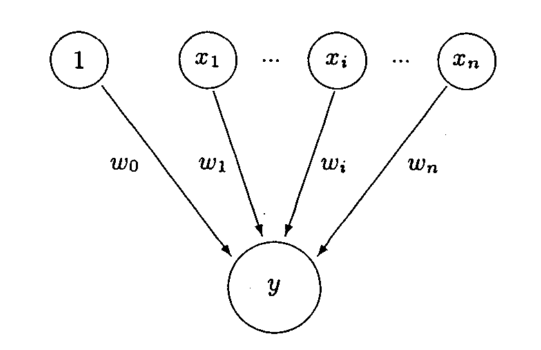
\includegraphics[width=0.7\linewidth]{perceptron.png} 
\end{center}	   
\caption{Mechanism of a Perceptron}\label{perceptron_fig}
\end{figure}

\noindent The output of a perceptron is computed as:
\begin{equation}
	y=w_0+\sum _{i=1}^{n}x_i w_i
\end{equation}
Similar to Perceptron Branch Predictor(PBP), PBNBP is also based on perceptron, the simplest neural networks approach. Since dynamic branch predictors need to make decisions based on branch taken history, PBNBP keeps a global history shift register that records the outcomes of branches as they are executed or speculatively as they are predicted. In order to do this, it keeps an $ n\times (h+1)$ matrix $w_{n\times (h+1)}$ , in which every element is an 8-bit bytes integer weights, while $n$ is a design parameter. Each row of the matrix is an (h+1)-length weights vector, each vector stores the weights of one perceptron. The first weight elements of any row is known as the biased weight. The Boolean vector $g[1\dots h]\in \{1\dots h\}\times \{taken, not\_taken\}$ represents the global history shift register \cite{jimenez2001dynamic}. Different from PBP, only the bias weight in PBNBP is used to predict the current branch. The bias weight is added to a taken total of last $h$ branches, with each summand added during the processing of a previous branch \cite{jimenez2003fast}. 


\subsection{Algorithm}
Different from the original paper, we propose our detailed algorithm for both prediction and perceptron updating. These two algorithms are proposed in Algo \ref{predict_algo} and Algo \ref{update_algo}, respectively. Symbols in our algorithm are explained in Table \ref{symbol_tb}. Since the algorithm listed below is in detail and self-explanatory, we skipped the description part here.


\begin{algorithm}[!htp]
  \caption{\textsc{Predictor Update}}
  \label{update_algo}
  \begin{algorithmic}
  \Function{Update}{update, outcome}
	\State $prediction=update.prediction$
	\State $y=update.y$
	\State $i=update.i$
	\For{$j=1\rightarrow h$}
		\State $k=h-j$
		\If{$outcome==taken$}
			\State $r[k+1]=r[k]+w[i, j]$
		\Else
			\State $r[k+1]=r[k]-w[i, j]$
		\EndIf
	\EndFor
	\State $r[0]=0$
	\State $shift(g, outcome)$
	\State $shift(v, i)$

	\If{$outcome\neq prediction$}
		\State $sr=r$
		\State $sg=g$
		\State $sv=v$
	\EndIf

	\If{$outcome\neq prediction\|abs(y)<\theta $}
		\State $p\_update(w[i, 0], outcome)$
		\For{$j=1\rightarrow h$}
			\State $k=update.v[j]$
			\State $flag=(outcome==update.h[j])$
			\State $w[k, j]=p\_update(w[k, j], flag)$
		\EndFor
	\EndIf
  \EndFunction
  \end{algorithmic}
\end{algorithm}


\section{Evaluation}
\subsection{Misprediction Recovery}
Similar to the original paper, our implementation also includes a misprediction recovery mechanism to prevent critical errors caused by misprediction. As mentioned in Table, there are several symbols with prefix ``s'', meaning speculative, those are the speculative version of historical predicted branch address array, historical prediction partial sum array, etc. What we do in the algorithms using those speculative arrays is as follows:
\begin{itemize}
	\item After the branch prediction, the speculative branch outcome, global history register and partial sums are recorded in speculative arrays.
	\item When doing branch predictions before historical outcomes are available, i.e., historical branches executed, we use speculative arrays as historical records as input.
	\item If certain branches finished execution, we check if we do branch prediction wrong, and update speculative arrays to non-speculative results accordingly.
\end{itemize}
Through those approaches, the resilience of our branch predictor is guaranteed and the delay of waiting historical branches to finish is greatly reduced.

\subsection{Latency}
Comparing to the Java implementation \cite{javapathpre} of the path-based neural predictor, we exploit several features of C++ to reduce the prediction latency:
\begin{itemize}
	\item {\bf memset: }The initialization process of the neural predictor is time-consuming, especially when we are using a long history length for high prediction accuracy. Different from the loop-assign process in the Java implementation, we exploit memset in C++ which is much faster in setting the init value of weight matrix and other arrays.
	\item {\bf memcpy: }Noticing a large portion of shift and array copy operations conducted in the predictor, we use memcpy to perform those so that the performance is optimized.
\end{itemize}


\begin{figure}[htbp]
\begin{center}
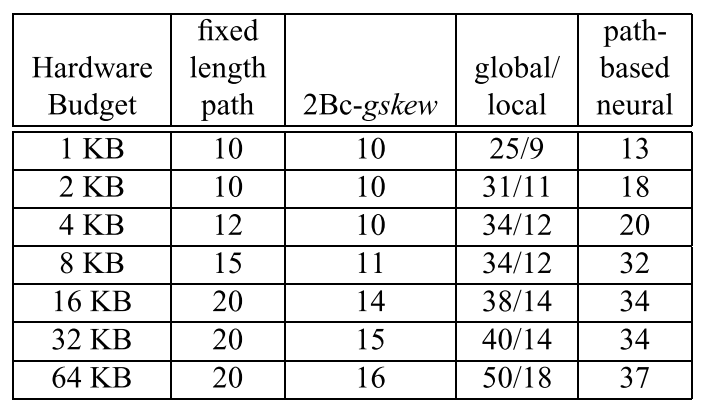
\includegraphics[width=\linewidth]{history_length.png} 
\end{center}	   
\caption{Tuned History Length}\label{history_length}
\end{figure}

\subsection{Hardware Budget}
The major memory consumption of path based neural predictor comes from its weight matrix, which contains in total $n\times (h+1)$ entries. As a common practice, we use 8 bits for one entry in the matrix, which means the weight range in our implementation is $[-128, 127]$. Under this setting, we referred to Fig. \ref{history_length} in \cite{jimenez2003fast} and discover that under 8KB budget the best choice of history length is 32(which also informs us that $n=256$). Therefore, the hardware budget is set according to the original paper and certified to meet the project requirements.

\subsection{Misprediction Rate}
Fig. shows the misprediction rates for our branch predictor ranging over hardware budgets from 1KB to 64 KB based on the provided microarchitectural instrastructure. Clearly, our predictor performs very well since even the least 1KB budget (history length 13) using our predictor can produce a much better result than 32,768-entry \emph{gshare} with history length of 15.

\begin{figure}[htbp]
\begin{center}
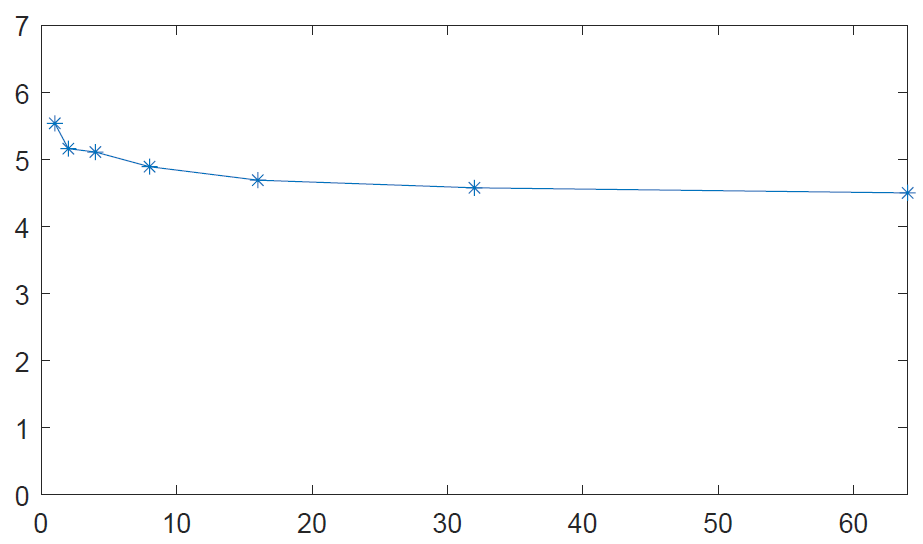
\includegraphics[width=\linewidth]{results.png} 
\end{center}	   
\caption{Misprediction Rate Per Hardware Budget}\label{results}
\end{figure}



% An example of a floating figure using the graphicx package.
% Note that \label must occur AFTER (or within) \caption.
% For figures, \caption should occur after the \includegraphics.
% Note that IEEEtran v1.7 and later has special internal code that
% is designed to preserve the operation of \label within \caption
% even when the captionsoff option is in effect. However, because
% of issues like this, it may be the safest practice to put all your
% \label just after \caption rather than within \caption{}.
%
% Reminder: the "draftcls" or "draftclsnofoot", not "draft", class
% option should be used if it is desired that the figures are to be
% displayed while in draft mode.
%
%\begin{figure}[!t]
%\centering
%\includegraphics[width=2.5in]{myfigure}
% where an .eps filename suffix will be assumed under latex, 
% and a .pdf suffix will be assumed for pdflatex; or what has been declared
% via \DeclareGraphicsExtensions.
%\caption{Simulation results for the network.}
%\label{fig_sim}
%\end{figure}

% Note that the IEEE typically puts floats only at the top, even when this
% results in a large percentage of a column being occupied by floats.


% An example of a double column floating figure using two subfigures.
% (The subfig.sty package must be loaded for this to work.)
% The subfigure \label commands are set within each subfloat command,
% and the \label for the overall figure must come after \caption.
% \hfil is used as a separator to get equal spacing.
% Watch out that the combined width of all the subfigures on a 
% line do not exceed the text width or a line break will occur.
%
%\begin{figure*}[!t]
%\centering
%\subfloat[Case I]{\includegraphics[width=2.5in]{box}%
%\label{fig_first_case}}
%\hfil
%\subfloat[Case II]{\includegraphics[width=2.5in]{box}%
%\label{fig_second_case}}
%\caption{Simulation results for the network.}
%\label{fig_sim}
%\end{figure*}
%
% Note that often IEEE papers with subfigures do not employ subfigure
% captions (using the optional argument to \subfloat[]), but instead will
% reference/describe all of them (a), (b), etc., within the main caption.
% Be aware that for subfig.sty to generate the (a), (b), etc., subfigure
% labels, the optional argument to \subfloat must be present. If a
% subcaption is not desired, just leave its contents blank,
% e.g., \subfloat[].


% An example of a floating table. Note that, for IEEE style tables, the
% \caption command should come BEFORE the table and, given that table
% captions serve much like titles, are usually capitalized except for words
% such as a, an, and, as, at, but, by, for, in, nor, of, on, or, the, to
% and up, which are usually not capitalized unless they are the first or
% last word of the caption. Table text will default to \footnotesize as
% the IEEE normally uses this smaller font for tables.
% The \label must come after \caption as always.
%
%\begin{table}[!t]
%% increase table row spacing, adjust to taste
%\renewcommand{\arraystretch}{1.3}
% if using array.sty, it might be a good idea to tweak the value of
% \extrarowheight as needed to properly center the text within the cells
%\caption{An Example of a Table}
%\label{table_example}
%\centering
%% Some packages, such as MDW tools, offer better commands for making tables
%% than the plain LaTeX2e tabular which is used here.
%\begin{tabular}{|c||c|}
%\hline
%One & Two\\
%\hline
%Three & Four\\
%\hline
%\end{tabular}
%\end{table}


% Note that the IEEE does not put floats in the very first column
% - or typically anywhere on the first page for that matter. Also,
% in-text middle ("here") positioning is typically not used, but it
% is allowed and encouraged for Computer Society conferences (but
% not Computer Society journals). Most IEEE journals/conferences use
% top floats exclusively. 
% Note that, LaTeX2e, unlike IEEE journals/conferences, places
% footnotes above bottom floats. This can be corrected via the
% \fnbelowfloat command of the stfloats package.




\section{Conclusion}
We have presented a new implementation of path-based neural branch predictor. The predictor is originally proposed in \cite{jimenez2003fast} as an improvement of initial neural branch predictor in \cite{jimenez2001dynamic}, its Java implementation can be found at \cite{javapathpre}. The programming language is C++ and we exploited several C++ features to improve the predictor's latency. We also presented a comprehensive test of the branch predictor built on different hardware budget, experimental results showed that it achieves a miss rate of  4.893\% under the project specified 8KB budget, which is 22.4\% lower than \emph{gshare}'s 6.305\%. Moreover, with the increase of hardware budget, it can achieve even better performance, e.g., 4.578\% miss rate under 32KB budget.




% conference papers do not normally have an appendix


% use section* for acknowledgment





% trigger a \newpage just before the given reference
% number - used to balance the columns on the last page
% adjust value as needed - may need to be readjusted if
% the document is modified later
%\IEEEtriggeratref{8}
% The "triggered" command can be changed if desired:
%\IEEEtriggercmd{\enlargethispage{-5in}}

% references section

% can use a bibliography generated by BibTeX as a .bbl file
% BibTeX documentation can be easily obtained at:
% http://mirror.ctan.org/biblio/bibtex/contrib/doc/
% The IEEEtran BibTeX style support page is at:
% http://www.michaelshell.org/tex/ieeetran/bibtex/
%\bibliographystyle{IEEEtran}
% argument is your BibTeX string definitions and bibliography database(s)
%\bibliography{IEEEabrv,../bib/paper}
%
% <OR> manually copy in the resultant .bbl file
% set second argument of \begin to the number of references
% (used to reserve space for the reference number labels box)
\bibliographystyle{IEEEtran}
% argument is your BibTeX string definitions and bibliography database(s)
\bibliography{refs}




% that's all folks
\end{document}


